Считывающая электроника жидкаргоновых калориметров детектора ATLAS имеет сложную структуру, но в самом верхнем уровне её можно разделить на 2 части: фронтенд и задетекторную электронику. На рис. \ref{fig:read_electronics} изображена общая схема устройства считывающей электроники системы жидкоаргоновы калориметров.
\begin{figure}[ht]
    \centering
    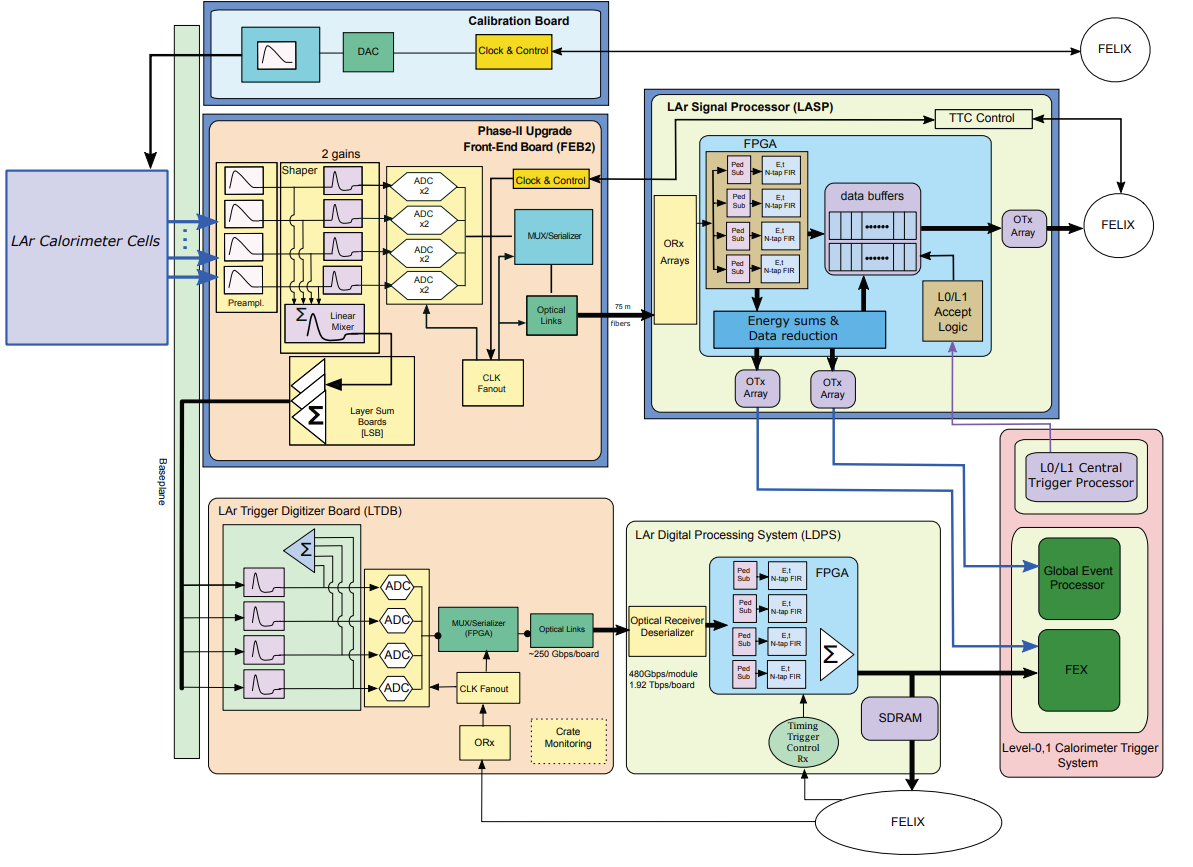
\includegraphics[width=\linewidth]{read_electronics.png}
    \caption{Схема считывающей электроники жидкоаргоновых калориметров ATLAS}
    \label{fig:read_electronics}
\end{figure}\par
Фронтенд часть располагается в непосредственной близости с ускорителем, поэтому на неё налагаются определённые требования по радиационной стойкости и отказоустойчивости. В рамках второй фазы обновления электроники на детектор будут установлены новые платы считывания FEB2(FEB -- Front-End Board), а также платы калибровки.\par

\subsubsection{Модуль FEB2}
Платы FEB2 принимают сигналы от калориметрических ячеек и выполняют их аналоговую обработку, включая усиление, формирование и разделение на две перекрывающиеся шкалы линейного усиления. Обе шкалы усиления оцифровываются при помощи 14-битного АЦП, после чего цифровые синалы сериализуются и отправляются через оптический канал связи. Для этого используется несколько специализированных интегральных микросхем, а также системы управления и синхронизации. Каждая плата FEB2 способна обрабатывать 128 калориметрических каналов, а для считывания всей системы жидкоаргоновых калориметров требуется 1524 таких устройств.\par


\subsubsection{Модуль LTDB}
\input{subsections/ltdb.tex}

\subsubsection{Калибровочная система}
Важной частью фронтенд электроники является калибровочная система. С помощью специальных плат реализуется подача точных калибровочных сигналов непосредственно на ячейки жидкоаргонового калориметра. Форма калибровочного сингала максимально приближена к импульсу ионизации, генерируемому электромагнитным ливнем в детекторе. В силу того, что получить истинно треугольный сигнал с помощью электронной схемы достаточно трудно, первоначально создаётся экспоненциальный импульс, у которого обрезается область затухания для максимального приближения к желаемой треугольной форме, по крайней мере, в начальной части импульса. Для компенсации остаточной разницы в форме между физическим импульсом ионизации и калибровочным сигналом производится непосредственное измерение свойств последнего для их учёта в процедуре калибровки.\par


